% Options for packages loaded elsewhere
\PassOptionsToPackage{unicode}{hyperref}
\PassOptionsToPackage{hyphens}{url}
\PassOptionsToPackage{dvipsnames,svgnames,x11names}{xcolor}
%
\documentclass[
  12pt,
  a4paper,
  DIV=11,
  numbers=noendperiod]{scrartcl}

\usepackage{amsmath,amssymb}
\usepackage{lmodern}
\usepackage{setspace}
\usepackage{iftex}
\ifPDFTeX
  \usepackage[T1]{fontenc}
  \usepackage[utf8]{inputenc}
  \usepackage{textcomp} % provide euro and other symbols
\else % if luatex or xetex
  \usepackage{unicode-math}
  \defaultfontfeatures{Scale=MatchLowercase}
  \defaultfontfeatures[\rmfamily]{Ligatures=TeX,Scale=1}
\fi
% Use upquote if available, for straight quotes in verbatim environments
\IfFileExists{upquote.sty}{\usepackage{upquote}}{}
\IfFileExists{microtype.sty}{% use microtype if available
  \usepackage[]{microtype}
  \UseMicrotypeSet[protrusion]{basicmath} % disable protrusion for tt fonts
}{}
\makeatletter
\@ifundefined{KOMAClassName}{% if non-KOMA class
  \IfFileExists{parskip.sty}{%
    \usepackage{parskip}
  }{% else
    \setlength{\parindent}{0pt}
    \setlength{\parskip}{6pt plus 2pt minus 1pt}}
}{% if KOMA class
  \KOMAoptions{parskip=half}}
\makeatother
\usepackage{xcolor}
\usepackage[top=30mm,left=20mm,right=20mm,bottom=30mm,heightrounded]{geometry}
\setlength{\emergencystretch}{3em} % prevent overfull lines
\setcounter{secnumdepth}{5}
% Make \paragraph and \subparagraph free-standing
\ifx\paragraph\undefined\else
  \let\oldparagraph\paragraph
  \renewcommand{\paragraph}[1]{\oldparagraph{#1}\mbox{}}
\fi
\ifx\subparagraph\undefined\else
  \let\oldsubparagraph\subparagraph
  \renewcommand{\subparagraph}[1]{\oldsubparagraph{#1}\mbox{}}
\fi

\usepackage{color}
\usepackage{fancyvrb}
\newcommand{\VerbBar}{|}
\newcommand{\VERB}{\Verb[commandchars=\\\{\}]}
\DefineVerbatimEnvironment{Highlighting}{Verbatim}{commandchars=\\\{\}}
% Add ',fontsize=\small' for more characters per line
\usepackage{framed}
\definecolor{shadecolor}{RGB}{241,243,245}
\newenvironment{Shaded}{\begin{snugshade}}{\end{snugshade}}
\newcommand{\AlertTok}[1]{\textcolor[rgb]{0.68,0.00,0.00}{#1}}
\newcommand{\AnnotationTok}[1]{\textcolor[rgb]{0.37,0.37,0.37}{#1}}
\newcommand{\AttributeTok}[1]{\textcolor[rgb]{0.40,0.45,0.13}{#1}}
\newcommand{\BaseNTok}[1]{\textcolor[rgb]{0.68,0.00,0.00}{#1}}
\newcommand{\BuiltInTok}[1]{\textcolor[rgb]{0.00,0.23,0.31}{#1}}
\newcommand{\CharTok}[1]{\textcolor[rgb]{0.13,0.47,0.30}{#1}}
\newcommand{\CommentTok}[1]{\textcolor[rgb]{0.37,0.37,0.37}{#1}}
\newcommand{\CommentVarTok}[1]{\textcolor[rgb]{0.37,0.37,0.37}{\textit{#1}}}
\newcommand{\ConstantTok}[1]{\textcolor[rgb]{0.56,0.35,0.01}{#1}}
\newcommand{\ControlFlowTok}[1]{\textcolor[rgb]{0.00,0.23,0.31}{#1}}
\newcommand{\DataTypeTok}[1]{\textcolor[rgb]{0.68,0.00,0.00}{#1}}
\newcommand{\DecValTok}[1]{\textcolor[rgb]{0.68,0.00,0.00}{#1}}
\newcommand{\DocumentationTok}[1]{\textcolor[rgb]{0.37,0.37,0.37}{\textit{#1}}}
\newcommand{\ErrorTok}[1]{\textcolor[rgb]{0.68,0.00,0.00}{#1}}
\newcommand{\ExtensionTok}[1]{\textcolor[rgb]{0.00,0.23,0.31}{#1}}
\newcommand{\FloatTok}[1]{\textcolor[rgb]{0.68,0.00,0.00}{#1}}
\newcommand{\FunctionTok}[1]{\textcolor[rgb]{0.28,0.35,0.67}{#1}}
\newcommand{\ImportTok}[1]{\textcolor[rgb]{0.00,0.46,0.62}{#1}}
\newcommand{\InformationTok}[1]{\textcolor[rgb]{0.37,0.37,0.37}{#1}}
\newcommand{\KeywordTok}[1]{\textcolor[rgb]{0.00,0.23,0.31}{#1}}
\newcommand{\NormalTok}[1]{\textcolor[rgb]{0.00,0.23,0.31}{#1}}
\newcommand{\OperatorTok}[1]{\textcolor[rgb]{0.37,0.37,0.37}{#1}}
\newcommand{\OtherTok}[1]{\textcolor[rgb]{0.00,0.23,0.31}{#1}}
\newcommand{\PreprocessorTok}[1]{\textcolor[rgb]{0.68,0.00,0.00}{#1}}
\newcommand{\RegionMarkerTok}[1]{\textcolor[rgb]{0.00,0.23,0.31}{#1}}
\newcommand{\SpecialCharTok}[1]{\textcolor[rgb]{0.37,0.37,0.37}{#1}}
\newcommand{\SpecialStringTok}[1]{\textcolor[rgb]{0.13,0.47,0.30}{#1}}
\newcommand{\StringTok}[1]{\textcolor[rgb]{0.13,0.47,0.30}{#1}}
\newcommand{\VariableTok}[1]{\textcolor[rgb]{0.07,0.07,0.07}{#1}}
\newcommand{\VerbatimStringTok}[1]{\textcolor[rgb]{0.13,0.47,0.30}{#1}}
\newcommand{\WarningTok}[1]{\textcolor[rgb]{0.37,0.37,0.37}{\textit{#1}}}

\providecommand{\tightlist}{%
  \setlength{\itemsep}{0pt}\setlength{\parskip}{0pt}}\usepackage{longtable,booktabs,array}
\usepackage{calc} % for calculating minipage widths
% Correct order of tables after \paragraph or \subparagraph
\usepackage{etoolbox}
\makeatletter
\patchcmd\longtable{\par}{\if@noskipsec\mbox{}\fi\par}{}{}
\makeatother
% Allow footnotes in longtable head/foot
\IfFileExists{footnotehyper.sty}{\usepackage{footnotehyper}}{\usepackage{footnote}}
\makesavenoteenv{longtable}
\usepackage{graphicx}
\makeatletter
\def\maxwidth{\ifdim\Gin@nat@width>\linewidth\linewidth\else\Gin@nat@width\fi}
\def\maxheight{\ifdim\Gin@nat@height>\textheight\textheight\else\Gin@nat@height\fi}
\makeatother
% Scale images if necessary, so that they will not overflow the page
% margins by default, and it is still possible to overwrite the defaults
% using explicit options in \includegraphics[width, height, ...]{}
\setkeys{Gin}{width=\maxwidth,height=\maxheight,keepaspectratio}
% Set default figure placement to htbp
\makeatletter
\def\fps@figure{htbp}
\makeatother

\usepackage{booktabs}
\usepackage{longtable}
\usepackage{array}
\usepackage{multirow}
\usepackage{wrapfig}
\usepackage{float}
\usepackage{colortbl}
\usepackage{pdflscape}
\usepackage{tabu}
\usepackage{threeparttable}
\usepackage{threeparttablex}
\usepackage[normalem]{ulem}
\usepackage{makecell}
\usepackage{xcolor}
\KOMAoption{captions}{tableheading}
\usepackage[none]{hyphenat} \usepackage[danish]{babel} \usepackage{dcolumn} \usepackage{threeparttable} \usepackage{fancyhdr}
\makeatletter
\makeatother
\makeatletter
\makeatother
\makeatletter
\@ifpackageloaded{caption}{}{\usepackage{caption}}
\AtBeginDocument{%
\ifdefined\contentsname
  \renewcommand*\contentsname{Table of contents}
\else
  \newcommand\contentsname{Table of contents}
\fi
\ifdefined\listfigurename
  \renewcommand*\listfigurename{List of Figures}
\else
  \newcommand\listfigurename{List of Figures}
\fi
\ifdefined\listtablename
  \renewcommand*\listtablename{List of Tables}
\else
  \newcommand\listtablename{List of Tables}
\fi
\ifdefined\figurename
  \renewcommand*\figurename{Figure}
\else
  \newcommand\figurename{Figure}
\fi
\ifdefined\tablename
  \renewcommand*\tablename{Table}
\else
  \newcommand\tablename{Table}
\fi
}
\@ifpackageloaded{float}{}{\usepackage{float}}
\floatstyle{ruled}
\@ifundefined{c@chapter}{\newfloat{codelisting}{h}{lop}}{\newfloat{codelisting}{h}{lop}[chapter]}
\floatname{codelisting}{Listing}
\newcommand*\listoflistings{\listof{codelisting}{List of Listings}}
\makeatother
\makeatletter
\@ifpackageloaded{caption}{}{\usepackage{caption}}
\@ifpackageloaded{subcaption}{}{\usepackage{subcaption}}
\makeatother
\makeatletter
\@ifpackageloaded{tcolorbox}{}{\usepackage[many]{tcolorbox}}
\makeatother
\makeatletter
\@ifundefined{shadecolor}{\definecolor{shadecolor}{rgb}{.97, .97, .97}}
\makeatother
\makeatletter
\makeatother
\ifLuaTeX
  \usepackage{selnolig}  % disable illegal ligatures
\fi
\IfFileExists{bookmark.sty}{\usepackage{bookmark}}{\usepackage{hyperref}}
\IfFileExists{xurl.sty}{\usepackage{xurl}}{} % add URL line breaks if available
\urlstyle{same} % disable monospaced font for URLs
\hypersetup{
  pdftitle={Projekt hos Thise Mejeri},
  pdfauthor={Kenneth Gottfredsen, Eva Rauff og Sanne Sørensen},
  colorlinks=true,
  linkcolor={blue},
  filecolor={Maroon},
  citecolor={Blue},
  urlcolor={Blue},
  pdfcreator={LaTeX via pandoc}}

\title{Projekt hos Thise Mejeri}
\usepackage{etoolbox}
\makeatletter
\providecommand{\subtitle}[1]{% add subtitle to \maketitle
  \apptocmd{\@title}{\par {\large #1 \par}}{}{}
}
\makeatother
\subtitle{Et datamodenhedsprojekt der undersøger sammenhængen mellem
vejret og efterspørgslen på koldskål}
\author{Kenneth Gottfredsen, Eva Rauff og Sanne Sørensen}
\date{1/2/23}

\begin{document}
\maketitle
\ifdefined\Shaded\renewenvironment{Shaded}{\begin{tcolorbox}[boxrule=0pt, breakable, borderline west={3pt}{0pt}{shadecolor}, enhanced, sharp corners, frame hidden, interior hidden]}{\end{tcolorbox}}\fi

\renewcommand*\contentsname{Indholdsfortegnelse}
{
\hypersetup{linkcolor=}
\setcounter{tocdepth}{3}
\tableofcontents
}
\setstretch{1.5}
\setcounter{page}{1} 
\parindent 0ex
\emergencystretch 3em
\pagestyle{fancy}
\fancyhead{}
\fancyfoot{}
\fancyfoot[C]{\thepage}
\renewcommand{\headrulewidth}{0.5pt}
\renewcommand{\footrulewidth}{0.5pt}

\hypertarget{problemfelt}{%
\section{Problemfelt}\label{problemfelt}}

Det er vanskeligt at forudsige hvor meget koldskål Thise skal producere
til deres kunder (Kjer 2022). Sommervejret påvirker kundernes
efterspørgsel på koldskål (Holland 2022). Hos Thise Mejeri bruger
medarbejderne vejrudsigten, og mange års erfaring når de skal vurdere,
hvor mange ltr. koldskål, der skal produceres (Jensen 2022). I en
artikel fra TV Midtvest fortæller adm. direktør Poul Pedersen fra Thise
Mejeri at: \emph{``Vi kigger på tal og vejrudsigter som aldrig før. Så
beslutter vi os for et tal, og vi plejer at være gode til at gætte.'' -
(ibid).} Det er et erhvervsøkonomisk problem, hvis man udelukkende
bruger vejrudsigten og gætteri til, at forudsige hvor meget koldskål
produktionsafdelingen skal producere. Gætteriet medfører en vis risiko,
da man ikke kan garantere, at alt koldskålen bliver solgt - selv når
vejret er godt! (ibid). Konsekvensen kan føre til et stort økonomisk
tab, fordi den mængde koldskål, som ikke bliver solgt i butikkerne,
leveres tilbage til Thises eget lager igen. Afhænger COOPs efterspørgsel
på koldskål kun af vejret? Er der andre mekanismer end vejret, som
forårsager en stigende eller faldende efterspørgsel på koldskål?
Formålet med undersøgelsen er, at undersøge hvordan Thises
datamodenhedsproces hænger sammen med COOPs efterspørgsel på koldskål.
Undersøgelsen bidrager med en multibel lineær regressionsmodel, som kan
give en tilnærmelsesvis præcis forudsigelse af, hvor mange ltr. koldskål
COOP vil efterspørge fremadrettet.

\hypertarget{problemformulering}{%
\section{Problemformulering}\label{problemformulering}}

På baggrund af ovenstående problemfelt bliver der i næste afsnit
formuleret et hovedspørgsmål og nogle underspørgsmål, de skal besvare
den erhvervsøkonomiske problemstillingen.

\hypertarget{hovedspuxf8rgsmuxe5l}{%
\subsection{Hovedspørgsmål}\label{hovedspuxf8rgsmuxe5l}}

\emph{``Hvordan kan Thises produktionsafdeling forbedre deres
datamodenhed og dermed forbedre udnyttelsen af deres egne data til
produktionsplanlægning?''}

\hypertarget{underspuxf8rgsmuxe5l-1}{%
\subsection{Underspørgsmål 1}\label{underspuxf8rgsmuxe5l-1}}

\emph{``Hvor befinder Thises produktionsafdeling sig på nuværende
tidspunkt datamodenhedsmæssigt?''}

\hypertarget{underspuxf8rgsmuxe5l-2}{%
\subsection{Underspørgsmål 2}\label{underspuxf8rgsmuxe5l-2}}

\emph{``Hvilke faktorer påvirker COOPs efterspørgsel af koldskål?''}

\hypertarget{underspuxf8rgsmuxe5l-3}{%
\subsection{Underspørgsmål 3}\label{underspuxf8rgsmuxe5l-3}}

\emph{``Hvilken model kan Thises produktionsafdeling bruge til at
forudsige COOPs efterspørgsel af koldskål fremadrettet?''}

\hypertarget{underspuxf8rgsmuxe5l-4}{%
\subsection{Underspørgsmål 4}\label{underspuxf8rgsmuxe5l-4}}

\emph{``Kan undersøgelsens resultater anvendes til at styrke
produktionsplanlægningen?''}

\hypertarget{videnskabsteori}{%
\section{Videnskabsteori}\label{videnskabsteori}}

Et paradigme er et tankesystem (Bergfors 2021). Sammenhængen mellem
Thises datamodenhedsproces, vejrforholdene og efterspørgslen af koldskål
er kompleks. Der er derfor behov for både kvalitativ og kvantitativ
viden til, at besvare problemstillingen.

Undersøgelsen styrer hen mod det \emph{realistiske} paradigme, fordi
tilgangen både fokuserer på tal og sproget. Formålet er at forklare
sammenhængene med tal, og dermed beskrive, forklare og forstå hvorfor
tallene ser ud, som de gør. Antagelsen er at Thises datamodenshedsproces
hænger sammen med Coops efterspørgsmål på koldskål samt andre
vejr-variables effekter herpå. \emph{Ontologi} er antagelsen om, hvordan
man anskuer den verden, problemstillingen indgår i (Bergfors 2021). Den
ontologiske opfattelse er, at virkeligheden hos Thise Mejeri eksisterer
uafhængigt af medarbejdernes egne opfattelser, da sandheden om Thises
datamodenhed og efterspørgslen på koldskål forstås objektivt (Bergfors
2021). \emph{Epistemologi} handler om, hvordan man anskaffer viden om en
problemstilling. Undersøgelsen bruger både kvalitative og kvantitative
data som bruges i kombination med hinanden, da forklaringer skal kunne
generaliseres - dette kaldes for metodekombination (ibid)

\hypertarget{design}{%
\section{Design}\label{design}}

Et undersøgelsesdesign er en strategisk plan som skal besvare en
problemstilling ud fra empiriske data (Bergfors 2021). Vi anvender et
\emph{statisk} undersøgelsesdesign til, at besvare vores
problemstilling. Fordi designet i sig selv giver et her - og nu billede.
Variablerne måles og observeres fx. fra perioden 1/4/22-30/8/22, hvilket
er en specifik periode. Dertil undersøges relationen mellem vejrvariable
og efterspørgslen på koldskål i deres nuværende tilstand (ibid).
Designtypen er et \emph{casestudium}, fordi vores problemstilling tager
afsæt i en nutidig kontekst, og fordi et casestudie undersøger komplekse
sammenhænge i dybden (ibid). Casen omhandler Thise Mejeri som
virksomhed. Formålet er at \emph{beskrive} og \emph{forstå} det
komplekse samspil der hænger sammen med Thises datamodenhedsproces,
vejret og COOPs efterspørgsel på koldskål.

\hypertarget{metodologi}{%
\section{Metodologi}\label{metodologi}}

\emph{Metodologi} henviser til de forskellige metoder, man kan bruge til
at indsamle data (ibid). Der anvendes eksisterende kvantitative data til
en regressionsanalyse. Denne data skal skabe større forståelse for,
hvorfor forskellige vejr-variable påvirker Coops efterspørgsel af
koldskål. Der bruges eksisterende sekundære vejrdata hentet med en API
fra Danmarks meteorologiske instituttet (DMI), og produktionsdata om
koldskål hentet fra Thises VMI-system. Som supplement til de
kvantitative data kombineres der med nogle kvalitative data i form af to
semistrukturerede interviews med to informanter. Den ene informant
arbejder i produktionsafdelingen, og den anden arbejder i
salgsafdelingen. Formålet med den kvalitative data er, at disse
dybdegående oplysninger kan bruges til, og forstå datamodenhed ud fra et
subjektivt medarbejderperspektiv.

\hypertarget{forretningsmodel}{%
\section{Forretningsmodel}\label{forretningsmodel}}

Et business model canvas er et illustrativt og strategisk værktøj som
bruges til, at forstå hvordan en forretningsmodel skaber økonomisk værdi
(Ostervalder \& Pigneur 2010). Det bruges i denne sammenhæng til, at
forstå Thises forretningsmodel.

Thise Mejeri bruger et VMI system som salgskanal. Et VMI system er et
leverandørstyret system. COOP bestiller deres koldskål igennem dette
system, og Thise producere dernæst koldskålen og opbevarer det på deres
eget lager. Dernæst transportere de selv koldskålen ud til COOPs
butikker. Thise har en intern aftale med COOP om, at de skal have mindst
\(80\%\) af af produkterne på lageret. De resterende \(20\%\) supplerer
de op med vha. Pareto forecasting, som er et endnu et system i deres
salgskanal. 80/20 reglen fra Pareto fungerer som et management værktøj,
da Thise hele tiden skal tilpasse deres salgsstrategier for at
opretholde deres leveringsservice på ca. \(98\%\).

Pareto er et godt værktøj til, at sikre at Thise opnår forskellige
KPI-målsætninger. Problemet med Pareto er, at det er abonnementbaseret
og dyrt, fik vi fortalt af Bjarne som er senior demand planner (Justesen
2022: 59). Der er stor risiko forbundet ved, at have et VMI system.
Bliver et produkt ikke solgt, leveres det tilbage til Thises hovedlager,
hvor det registreres på en spild konto (ibid). Derfor er det vigtigt, at
have nogle pålidelige forecasting modeller der kan forudsige
efterspørgslen af produkter med stor præcision. Thise får nemlig først
betaling når varen er solgt i COOPs butikker. Det kræver et tæt
samarbejde, at have et VMI system kørende. Derfor er det vigtigt at
Thise overholder deres produktvilkår til COOP, da de er bundet af
klausulaftaler som kan medføre forskellige sanktioner af økonomisk
karakter, så frem de ikke overholdes. Stærke kunderelationer er vigtigt
i den her sammenhæng.

\hypertarget{datamodenhed}{%
\section{Datamodenhed}\label{datamodenhed}}

Alexandramodellen er en datamodenhedsmodel. Den bruges til at finde af
hvor langt en virksomhed er i datamodenhedsprocessen, og hvordan den kan
bruge forskellige strategier til og blive mere datadrevne (Bækby et. al
2017). Modellen bruges til at undersøge hvor datamodne Thise er på
nuværende tidspunkt.

Thise Mejeri er på nuværende tidspunkt i fase 1, da de registrerer data
for at skabe en forståelse og værdi for virksomhedens drift (ibid).
Produktionsplanlæggeren har via. Navision adgang til alt virksomhedsdata
som fx. lagerstyring og finansiel styring gennem deres Windows
styresystem. Dette er en on-premises-løsning. Navision er et ERP
softwaresystem. Det bruges til at styre virksomhedens
forretningsprocesser og dermed effektivisere driften. og kan dermed
planlægge fremtidig produktionen. At de anvender programmet direkte
gennem deres Windows styresystem gør virksomheden sårbar overfor
systemnedbrud, hvilket de oplever ca. 5 gange om året.
Kompetencemæssigt, ifølge Bjarne, har Thise Mejeri en brist, da de ikke
har ansat nogle medarbejdere med relevant analyse erfaring (Justesen
2022: 45). De er derfor afhængige af den eksterne udbydere til at
forecaste med de data, der bliver indsamlet.

Produktionsplanlæggeren har via. Navision adgang til alt
virksomhedsdata, og det køres gennem deres Windows styresystem, hvilket
er en on-premises-løsning. Navision er ERP software til at håndtere
økonomi data til og træffe beslutninger ud fra. og kan dermed planlægge
fremtidig produktionen. At de anvender programmet direkte gennem deres
Windows styresystem gør virksomheden sårbar overfor systemnedbrud,
hvilket de oplever ca 5 gange om året. Kompetencemæssigt, ifølge Bjarne,
har Thise Mejeri en brist da de ikke har ansat nogle medarbejder med
relevant analyse erfaring. De er derfor afhængige af den eksterne
udbydere til at forecaste med de data, der bliver indsamlet (ibid).

\hypertarget{dataanalysen}{%
\section{Dataanalysen}\label{dataanalysen}}

Thise Mejeri har i dag svært ved, at forecaste hvor stor efterspørgslen
bliver på Koldskål i løbet af deres koldskålssæson, som ca. løber i
ugerne 13-36. Thise Mejeri ønsker, at opretholde deres leverings service
på 98\% på alle de produkter de har lovet levering på fortæller Søren
Jensen.

\hypertarget{baggrund}{%
\subsection{Baggrund}\label{baggrund}}

Den kvantitative del af analysen er afgrænset til COOP butikker i
nærheden af Landbohøjskolen, hvis beliggenhed er i Københavnområdet.
Butikkerne afgiver ordre til Thises fjernlager, hvorefter koldskålen
bliver leveret ud til butikkerne.

\hypertarget{formuxe5l}{%
\subsection{Formål}\label{formuxe5l}}

Formålet med analysen er derfor, at udregne en multibel lineær
regressionsmodel som bedst kan forudsige butikkernes efterspørgsel på
koldskål i området omkring Landbohøjskolen. Derudover vil vi også finde
ud af, hvordan vejret og andre vejr-relateret faktorer påvirker
butikkernes efterspørgsel på koldskål. Tilgangen kan løse Thises
forretningsproblem. Undersøgelsens dataminingproblem går ud på, at
identificere de forskellige vejr-variablers effekt på
efterspørgspørgslen af koldskål.

\hypertarget{importer-data-til-r}{%
\subsection{Importer data til R:}\label{importer-data-til-r}}

Først importeres datasættet ind i R-Studio:

\hypertarget{tidying-og-transformering}{%
\subsection{Tidying og transformering}\label{tidying-og-transformering}}

Nu har vi fået indlæst datasættet. Det næste skridt er gøre strukturen i
vores dataframe nemmere at arbejde med og mere læsevenlig. Processen
kaldes for tidy data, det betyder at hver variabel har en kolonne, hver
observation en række, samt hver observationsenhed er i en tabel (Wickham
2022). Det gør analysearbejdet nemmere. Først rekodes nogle af
variablerne, så de stemmer overens med hvad der står i
opgavebesvarelsen. I nedestående kodestump rekodes og transformeres de
udvalgte variabler så de stemmer overens med eksamensbesvarelsen. Hele
kodestumpen vil blive kædet sammen med `pipe' funktionen'. Omkodningerne
gems i en ny dataframe som kaldes data1. I den næste del anvendes mutate
igen til, at lave en kolonne der hedder dag, den bliver omkodet til en
faktor. Dernæst koder vi date til et objekt med \texttt{ymd()}`
funktionen fra lubridate pakken. ``lubridate.week.start'' 1=mandag,
istedet for søndag som er standardindstillingerne i R.

For at indhente data fra DMI laves en HTTP GET-anmodning til en API fra
DMI. Vi skal bruge adgangen til at få de relevante vejr-variable som vi
senere skal bruge i vores analyse. API'en leverer til slut et objekt i
JSON format som bliver transformeret om til en dataframe i stedet for en
liste. Først bruges base\_url og info\_url til at anmode om vejrdata fra
DMI's API. req\_url bruges til at udvælge specifikke parametre fra
API´en.

I næste kodechunk vil vi transformere den data vi har hentet fra vores
API-kald til nogle mere brugbare data. Først bruges base\_url og dernæst
info\_url til at anmode om vejrdata fra DMI's API. req\_url bruges til
at udvælge specifikke parametre fra API´en. Derefter bruges
\texttt{pivot\_wider()} til at fordele variablerne ud i deres egne
separate kolonner. mutate-funktionen bruges til at konvertere kolonnen
målingstidspunkt til datoformat. \texttt{Separate()} bruges til at
opdele kolonnen målingstidspunkt i to separate kolonner som navngives
`date' og `time'. \texttt{Filter(str\_sub)}funktionen udvælger rækker,
der indeholder de første fire karakterer: ``12:0''.

I nedestående kode-chunk bruges \texttt{left\_join()} til at returnere
alle rækkerne fra x, samt alle kolonner langs x og y (Wickham 2022).
Udvalgte dataframes sammenkobles fra data1 og data2 til data3. Da alle
kolonnerne er lige lange, er der ingen missing værdier. Dernæst anvendes
mutate til, at oprette fire nye variabler i data3 kaldet
temp\_gt25\_3\_dage. \texttt{Lag()} er brugt til at lave variablerne,
som har opfanget forsinkede værdier fra temp1, temp2 og temp3.
Afslutningsvis dannes variablen `temp\_gt25\_3\_dage', som måler de dage
hvor der har været mere end 3 dage i træk med \textgreater= 25 grader.
Det er en dummyvariabel fordi der bruges \texttt{if\_else}. Relevante
variabler bliver beskrevet når der tolkes på modelparametre i
regressionsanalysen.

\hypertarget{datavisualisering-og-eksplorativ-analyse}{%
\subsection{Datavisualisering og eksplorativ
analyse}\label{datavisualisering-og-eksplorativ-analyse}}

Nu er data blevet gjort tidy. Næste skridt er at undersøge hvilke
faktorer der kan hænge sammen med butikkernes efterspørgslen af
koldskål. I afsnittet begynder den eksplorative analyse.
\texttt{geom\_density()} funktionen bruges til, at forstå fordelingen og
til at forudsige den forventede fordeling af efterspørgslen på koldskål.
Man kan se at at spredningen af observationerne er størst omkring 520
ltr, det er gennemsnittet. Observationerne er normalfordelte. At de er
normalfordelt er en fordel, fordi den lineære regressionsmodel er en
parametrisk test, hvor ét af kravene er data skal være normaltfordelt
(Hastie et.al 2021). At kravet er opfyldt gør model-parametrene er mere
pålidelige.

I følgende kode-chunk er der vist et boxplot. Det skal vise den
statistiske variationen ift. butikkens forventede lagerbeholdning og
efterspørgslen på koldskål. Man kan se at median-efterspørgslen stiger
når fra høj til lav forventet lagerbeholdning af koldskål. Det tyder på
at der er en signifikant sammenhæng mellem de 2 variabler.

I næste kode-chunk er der lavet et boxplot som viser fordelingen af
efterspørgslen i forhold til om 25\% af butikkerne er løbet tør for
kammerjunkere eller ej. På baggrund af plottet kan man se at hvis
butikkerne ikke har kammerjunkere på lageret så falder efterspørgslen.
Det betyder efterspørgslen på koldskål stiger hvis butikkerne er løbet
tør for kammerjunkere.

Forneden er et boxplot som viser sammenhængen mellem måned og
efterspørgslen af koldskål. Det er tydeligt at se at
median-efterspørgslen stiger fra april-juli hvorefter efterspørgslen
igen falder i august.

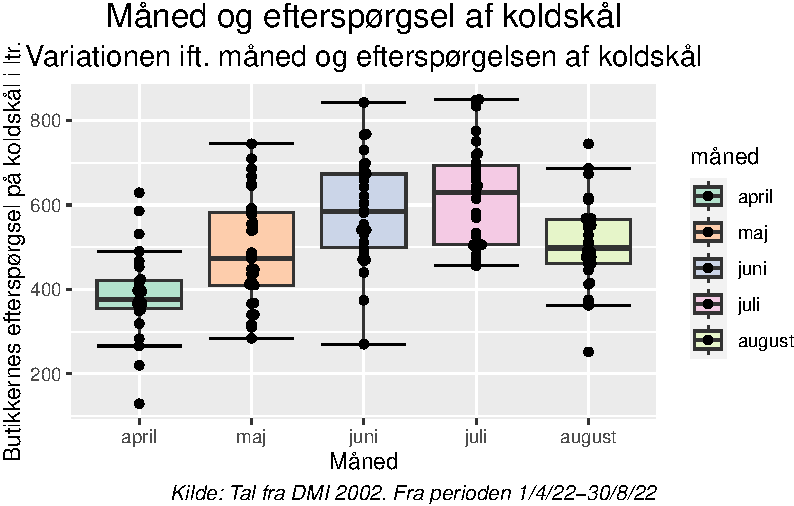
\includegraphics{Semester_projekt_2022_G1_files/figure-pdf/Chunk 10 - Boxplot over efterspørgsel og måned-1.pdf}

I nedestående kodechunk er der udvalgt 6 kontinuerte vejr-variabler,
fordi ønskes er, at undersøge om disse er korreleret med hinanden, og om
deres indbyrdes korrelation er statistisk signifikant. Der anvendes en
\texttt{chart.Correlation()} til at foretage en korrelationsanalyse.

Efterspørgel og humidity er ikke korreleret, og dermed ikke statistisk
signifikant. Beslutningen er derfor, at humidity ikke vil blive
inkluderet i analysen. Efterspørgsel og den gennemsnitlige temperatur
per time har en moderat korrelations koefficient på 0.38. P-værdien er
lav med tre stjerner, det betyder at sammenhængen er signifikant. Det er
derfor usandsynligt at opnå et mere ekstremt resultat, hvis man foretog
en ny undersøgelse. Mindre end \(5\%\) af korrelationen skyldes derfor
tilfældighed. Alle temperatur-variablerne er tæt på 1, hvilket betyder
at de har stærk samvariation. Dette kaldes for multikolinearitet. Det
vil sige, hvis de blev brugt i den endelige model ville det være
vanskeligt, at fortolke på koefficienterne. En Model med høj
multikolinearitet bliver mindre præcis og mindre pålidelig. For at
reducere multikolineariteten fjernes de øvrige temperatur-variable.

Som førnævnt var der en moderat signifikant sammenhæng mellem
efterspørgslen og gennemsnits temperaturen. Derfor bruges
temp\_mean\_past1h som den uafhængige effekt i næste kodechunk. Der
anvendes \texttt{predict()} til at konstruere et 95\(%
\) prædiktionsinterval, efterfulgt af \texttt{geom\_smooth()} til og
visualisere sammenhængen med et scatterplot.

Ud fra scatterplottet kan man se, at forholdet mellem den gennemsnitlige
temperatur og butikkernes efterspørgsel på koldskål er moderat lineært.
Fordi hældningen på tendenslinjen er positiv. Det antages at når
gennemsnits temperaturen stiger én enhed, vil efterspørgslen stige
tilsvarende, det `forholdsvis' mange af datapunkterne er placeret
omkring tendenslinjen. Der anvendes lineær regression, fordi det er en
simpel metode, og det er nemt at tolke på model-parametrene. Mange af
datapunkterne ligger også langt væk fra tendenslinjen, der udtrykker en
stigende gennemsnitlig efterspørgsel på koldskål i ltr. Det indikerer at
der er stor varians og potentiel bias tilstede. En mere kompleks model
kan derfor anvendes til, at forklare sammenhængen. Flere af
observationerne er placeret udenfor dette bånd, hvorfor det er besluttet
at anvende et prædiktionsinterval i stedet - der er den røde stiplede
linje. Formålet er med andre ord, at medregne usikkerheden omkring de
individuelle værdier og ikke usikkerheden omkring gennemsnittet. Når den
gennemsnitlige temperatur hver time er 30 °C, er efterspørgslen på
koldskål for én ny observation 629.87 ltr. Ved samme temperatur vil
butikkernes efterspørgslen af koldskål med 95\% sikkerhed være
{[}369.30:890.43{]}. Man kan på baggrund af nedestående figur tydeligt
se, at hvis den gennemsnitlige temperatur i °C stiger, stiger
butikkernes efterspørgsel på koldskål tilsvarende.

\begin{verbatim}
       fit      lwr      upr
1 440.6455 181.7817 699.5094
2 535.2564 278.2290 792.2838
3 629.8672 369.3044 890.4301
\end{verbatim}

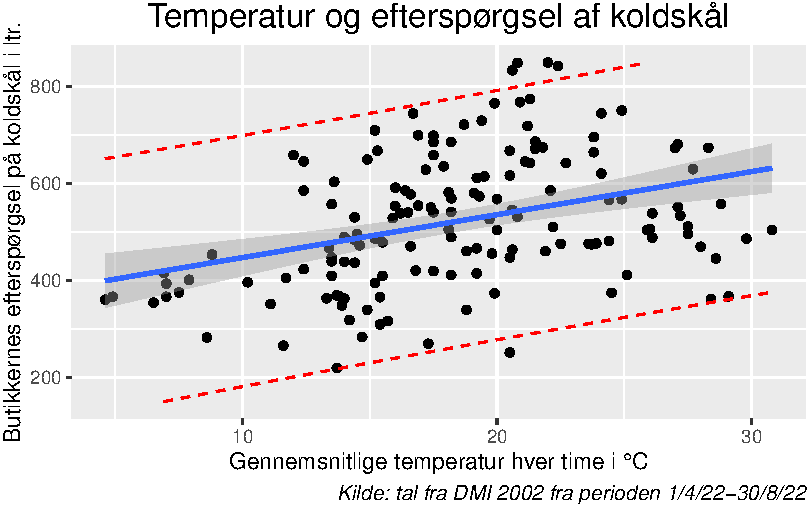
\includegraphics{Semester_projekt_2022_G1_files/figure-pdf/Chunk 12 - Scatterplot af temperatur og efterspørgsel-1.pdf}

\hypertarget{truxe6ning-puxe5-truxe6ningsdata}{%
\subsection{Træning på
træningsdata}\label{truxe6ning-puxe5-truxe6ningsdata}}

Først trænes modellen på træningsdata, fordi vi gerne vil tilpasse
modelparametrene. Der anvendes træningsdata til, at fintune vores
regressionsmodel. Efter modellen er blevet trænet godt igennem, bliver
den afprøvet på testdata, da man gerne vil undersøge hvor god modellen
er til, at forudsige en så præcis efterspørgsel på koldskål som mulig.
Vurderingen af modelpræcisionen bestemmes ud fra den laveste MSE værdi.
MSE måler hvor langt den forudsagte værdi for en observation er fra den
faktiske værdi for en observation. Er MSE lille er der den forudsagte
værdi tæt på den faktiske værdi, er MSE stor er den forudsagte værdi
langt fra den faktiske værdi. MSE er således et udtryk for, hvor præcis
den udvalgte model er til, at forudsige efterspørgslen af koldskål
(Hastie et.al 2021). MSE skal være så tæt på \(0\) som muligt.

Antallet af variabler i det samlede datasæt er mindre end antallet af
observationer. Derfor bruges backward-selection til, at udvælge de
uafhængige variabler som fremadrettet skal indgå i modellerne. Det vil
sige, at vi tilføjer alle variable ind på højre side af ligningen, og
fjerner dem med den højeste p-værdi indtil der kun er signifikante
uafhængige variable tilbage (Hastie et.al 2021). Denne teknik kan hjælpe
med at reducere unødvendig varians i den udvalgte model. men på samme
tid er den effektiv til, at identificere vigtige relationer i datasættet
(ibid).

\hypertarget{test-puxe5-testdata}{%
\subsection{Test på testdata}\label{test-puxe5-testdata}}

I det foregående afsnit blev den gennemsnitlige MSE beregnet for hver af
de fire modeller på træningsdata. Vi er egentlig ligeglade med disse MSE
værdier. Det er mere interessant at se hvor præcise forudsigelserne er
på testdata. Træningsdata anvendes som førnævnt til, at udvælge
signifikante uafhængige variable og tilpasse modelparametrene.

Dog er det værd at nævne, at den data undersøgelsen er baseret på
simulerede data. Dvs. at \(f\) er kendt allerede. Den virkelige sandhed
om efterspørgslen af koldskål vides dog ikke. Men hvis der bliver
udtrukket nogle testdata ud fra data3, kan man validere hvor godt en
model performer på disse testdata, når modelkompleksiteten øges.
Kompleksiteten kan øges ved, at de kontinuerte variable opløftes i flere
potenser, eller ved og inkludere flere uafhængige variabler.

\hypertarget{metode-til-test-af-model-performance}{%
\subsection{Metode til test af model
performance}\label{metode-til-test-af-model-performance}}

Man kan producere testdata på flere måder. Der anvendes en \emph{LOOCV}
metode, fordi data3 kun indeholder 151 observationer i alt. Fordelen ved
fremgangsmåden er, at den træner på alle observationerne, undtagen ét
datapunkt. Processen gentages i dette tilfælde 150 gange. Derefter
beregnes en gennemsnitlig MSE score, som udtrykker hvor god
modelpræcisionen er (Hastie et.al 2021). Problemet med metoden er, at
det kræver stor computerkraft, det er fordi modellen trænes k gange
(ibid).

\hypertarget{resultater}{%
\section{Resultater}\label{resultater}}

Nu er de fire modeller blevet trænet på træningsdata og testet godt
igennem på testdata. Resultaterne tager kun udgangspunkt i
koefficienterne fra de fire testmodeller. Modellen med den laveste
kvadrerede RMSE, og den højeste \(R^2\) er den model som har størst
præcision.

Baselinemodellen har kun den afhængige variabel i ligningen.
\(\hat{\beta_0}\) er den gennemsnitlige efterspørgsel på koldskål ved
\(520.23\) ltr. \(RMSEtest=139.20\). Bliver Temp\_mean\_past1h
inkluderet i den simple model, falder \(RMSEtest=130.36\), det betyder
at modellen `fitter' bedre på data og at modellen batter lidt mere.
Inkluderes de kategoriske faktorer i modellen med moderat kompleksitet,
falder \(RMSEtest=88.55\) . Det er den model hvor den forudsagte værdi
er tættest på den faktiske værdi. Dertil er \(adjR^2 = 0.63\%\), det
referer til den proportion af butikkernes efterspurgte koldskål som
bliver forklaret af de uafhængige variabler. De forklarer altså 63\% af
den samlede varians i datasættet.

Bliver modellen mere kompleks, bliver præcisionen ikke bedre - ofte
gælder det modsatte! I den komplekse model stiger \(RMSEtest=89.37\) og
\(adjR^2 = 0.62\%\), dvs. den begynder at falde. Desuden bliver
Temp\_mean\_past1h\^{}22 insignifikant, da hældningen er 0. Dette
skyldes muligvis overfitting.

Den moderate model er blevet udvalg til den mest præcise model.
Fortolkningen af koefficienterne er, når de øvrige variabler holdes
konstant:

\begin{itemize}
\item
  Er den forventede lagerbeholdning på mellemste niveau, falder
  butikkernes gennemsnitlige efterspørgsel på koldskål med \(-76.57\)
  ltr, i forhold til butikker med en lav forventet lagerbeholdningen.
\item
  Er den forventede lagerbeholdning på højeste niveau, falder
  butikkernes gennemsnitlige efterspørgsel på koldskål med \(-82.67\)
  ltr, i forhold til butikker med en lav forventet lagerbeholdning.
  Ændres referencegruppen, stiger efterspørgslen tilsvarende.
\end{itemize}

Det giver umiddelbart god mening, da butikkerne ikke vil risikere at
bestille for meget koldskål. Da der er risiko for, at den ikke bliver
solgt, og dermed øges riskoen for, at koldskålen overskrider sidste
salgsdato.

\begin{itemize}
\tightlist
\item
  Er 25\% af butikkerne i det pågældende område ikke løbet tør for
  kammerjunkere, falder butikkernes gennemsnitlige efterspørgsel med
  \(-71.89\) ltr, sammenlignet med de 25\% af butikkerne i det
  pågældende som er løbet tør for kammerjunkere. Ændres
  referencegruppen, stiger efterspørgslen tilsvarende.
\end{itemize}

Butikkerne vil gerne lave mersalg og dermed sælge kammerjunkere sammen
koldskål, det kan også indikere at forbrugerne synes koldskål og
kammerjunkere skal spises sammen.

\begin{itemize}
\tightlist
\item
  I maj måned stiger butikkernes efterspørgsel på koldskål
  gennemsnitligt med \(84.37\) ltr, i forhold til april måned. I juni
  måned stiger efterspørgslen gennemsnitligt med \(129.51\) ltr, i
  forhold til april måned. I juli måned stiger efterspørgslen
  gennemsnitligt med \(155.95\) ltr, i forhold til april måned. I august
  falder efterspørgslen ned til \(85.10\) ltr, sammenlignet med april
  måned.
\end{itemize}

Det betyder, at butikkernes gennemsnitlige efterspørgsel på koldskål
stiger hen over sommeren til og med august, hvor sæsonen nærmer sig
slutningen (Holland 2022)

\begin{itemize}
\tightlist
\item
  Har der været 25°C eller varmere i mere end tre dage, så falder
  butikkernes gennemsnitlige efterspørgsel på koldskål med \(-66.74\)
  ltr.
\end{itemize}

Det kan være en indikation på, at forbrugerne bliver trætte af at spise
koldskål, når det bliver for varmt over en længere periode.

\begin{itemize}
\tightlist
\item
  Stiger den gennemsnitlige temperatur målt pr. time med én °C, stiger
  butikkernes efterspørgsel på koldskål i gennemsnit med \(4.25\) ltr.
\end{itemize}

Øget sommervarme hænger moderat sammen med butikkernes efterspørgsel på
koldskål. Det stemmer overens med eksisterende viden på området (Kjer
2022).

\begin{longtable}[]{@{}
  >{\raggedright\arraybackslash}p{(\columnwidth - 8\tabcolsep) * \real{0.2990}}
  >{\centering\arraybackslash}p{(\columnwidth - 8\tabcolsep) * \real{0.1649}}
  >{\centering\arraybackslash}p{(\columnwidth - 8\tabcolsep) * \real{0.1649}}
  >{\centering\arraybackslash}p{(\columnwidth - 8\tabcolsep) * \real{0.1649}}
  >{\centering\arraybackslash}p{(\columnwidth - 8\tabcolsep) * \real{0.1753}}@{}}
\toprule()
\begin{minipage}[b]{\linewidth}\raggedright
\end{minipage} & \begin{minipage}[b]{\linewidth}\centering
\textbf{Baseline}
\end{minipage} & \begin{minipage}[b]{\linewidth}\centering
\textbf{Simpel}
\end{minipage} & \begin{minipage}[b]{\linewidth}\centering
\textbf{Moderat}
\end{minipage} & \begin{minipage}[b]{\linewidth}\centering
\textbf{Kompleks}
\end{minipage} \\
\midrule()
\endhead
\textbf{Forvent\_lager (mellem)} & & & \(-76.57\)\(***\)

\{\(19.82\)\} & \(-74.55\)\(***\)

\{\(19.72\)\} \\
\textbf{Forvent\_lager (høj)} & & & \(-82.67\)\(***\)

\{\(22.58\)\} & \(-87.00\)\(***\)

\{\(22.81\)\} \\
\textbf{Weekend\_helligdag (ja)} & & & \(113.01\)\(***\)

\{\(15.00\)\} & \(107.33\)\(***\)

\{\(15.16\)\} \\
\textbf{Kamjunk (nej)} & & & \(-71.89\)\(***\)

\{\(17.50\)\} & \(-76.52\)\(***\)

\{\(19.82\)\} \\
\textbf{Temp\_gt25\_3\_dage} & & & \(-82.00\)\(*\)

\{\(34.23\)\} & \(-66.74\)\(*\)

\{\(34.90\)\} \\
\textbf{Måned (maj)} & & & \(84.37\)\(***\)

\{\(24.54\)\} & \(101.69\)\(***\)

\{\(23.36\)\} \\
\textbf{Måned (juni)} & & & \(129.51\)\(***\)

\{\(32.79\)\} & \(162.71\)\(***\)

\{\(27.87\)\} \\
\textbf{Måned (juli)} & & & \(155.95\)\(***\)

\{\(32.79\)\} & \(155.947\)\(***\)

\{\(29.12\)\} \\
\textbf{Måned (august)} & & & \(85.10\)\(*\)

\{\(34.76\)\} & \(197.44\)\(*\)

\{\(30.96\)\} \\
\textbf{Temp\_mean\_past1h} & & \(9.46\)\(***\)

\{\(1.89\)\} & \(4.249\)\(*\)

\{\(2.07\)\} & \(0\) \\
Uafhængige variable & \(0\) & \(1\) & \(6\) & \(6\) \\
Skæring \(\hat{\beta_0}\) & \(520.23\)\(***\) & \(346.04\)\(***\) &
\(379.93\)\(***\) & \(434.78\)\(***\) \\
Model P-værdi & \(***\) & \(***\) & \(***\) & \(***\) \\
RMSE\_træning & \(139.20\) & \(128.74\) & \(82.10\) & \(83.21\) \\
RMSE\_test & \(139.20\) & \(130.36\) & \(88.55\) & \(89.37\) \\
\(R^2\) & & \(0.15\%\) & \(0.65\%\) & \(0.64\%\) \\
Justeret \(R^2\) & & \(0.14\%\) & \(0.63\%\) & \(0.62\%\) \\
Observationer & \(151\) & \(151\) & \(151\) & \(151\) \\
\bottomrule()
\end{longtable}

Tabel 1. Summeret modelreferat fra testdata. Referencegrupper () for
faktorerne er: kamjunkja, forvent\_lagerlav, månedapril. \{\} referer
til standardfejlen. Note:\(* = P < 0.1; ** = P < 0.05; *** = P <0.01\)

\hypertarget{diskussion}{%
\section{Diskussion}\label{diskussion}}

Først laves der et histogram med \texttt{ggplot()} der viser forskellen
i RMSE for alle modellerne på hhv. test og træningsdata ud fra
modelkomplesiteten. Forskellen i trænings- og test RMSE er jvf.
histogrammet ikke ens når kompleksiteten øges. I den simple model er
test-MSE'en større end trænings-MSE'en. Det samme mønster i den moderate
og den komplekse gælder. Det skyldes at vores SL-metode `tuner' modellen
for meget, så den køre modellen for hårdt på træningsdata. På den måde
opfanger modellen tilfældigheder fra træningsdata, i stedet for
egenskaber ved den \(f\), vi ikke kender til. Mønstret fra træningsdata
stemmer dermed ikke overens med mønstret i testdatasættet (Hastie 2022).
I histogrammet kan man også se, at forskellen mellem RMSE i den moderate
og den komplekse model er meget lille. Alt andet lige, vælges den
moderate ud fra et princip om sparsommelighed frem for den komplekse
model (ibid).

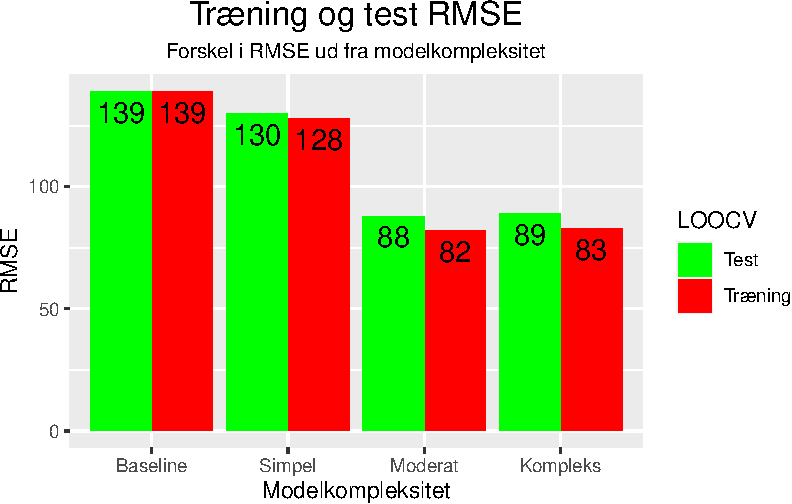
\includegraphics{Semester_projekt_2022_G1_files/figure-pdf/Chunk 15 - Histgram over MSE-1.pdf}

For det første hænger det optimale modeldevalg sammen med præcision i
forudsigelse og fortolkningen af parametrene. Stiger fleksibiliteten
bliver det svære at tolke på parametrene. Falder falder fleksibiliteten
bliver det nemmere at tolke på parametrene. Da Temp\_mean\_past1h blev
opløftet til Temp\_mean\_past1h\^{}22 i den komplekse model, blev p
værdien for \(\hat{\beta_1}\) for insignifikant ved \(Pr = 0.58\%\).
\(\hat{\beta_1}\) er derfor ikke tilstrækkelig langt fra \(0\). Dette
gjorde det vanskeligere at tolke på denne paramter. Det er fordi
modellen opfangede for mange fejl og for meget støj i form af bias.

For det andet hænger modelvalget sammen det bias/variance tradeoff som
forekommer, hvis man øger modelkompleksiteten i jagten på identificere
den model som har lavest varians og bias. Varians er ændringen i
\(\hat{f}\), når den beregnes på nye data - men værdien er aldrig helt
den samme! Stiger fleksibiliteten øges variansen. Bias opstår når man
forsøger, at forudsige et komplekst fænomen med en for simpel metode.
Stiger fleksibiliteten reduceres bias. Efterspørgslen på koldskål er som
førnævnt et multidimensionelt fænomen. Vi forsøgte at reducere bias ved
og udvide den simple lineære model med Temp\_mean\_past1h uden alle de
kategoriske faktorvariabler, da de ikke kan indgå i en polynomisk
regression. Det resulterede ikke i en forbedring i RMSE, eller en
stigning i \(R^2\). Hverken da den blev opløftet i 3 og 22 potens.
Valget blev derfor, at beholde faktorerne i den moderate model, fordi de
til sammen forklarer \(63\%\) af den samlede varians. Andre variable
kunne havde indflydelse på butikkernes efterspørgsel på koldskål.
Gennemsnitlige antal solskinstimer, maksimale vindhastighed, samt de
private forbrugers socioøkonomiske forhold kunne bidrage med flere
dimensioner til den moderate model. Beslutningen blev derfor, at vælge
den multible lineære model med moderat kompleksitet. I næste kapitel
udrulles anbefalingerne.

\hypertarget{anbefalinger}{%
\section{Anbefalinger}\label{anbefalinger}}

For at kunne designe og udvikle det bedste dataprodukt bruges et Data
Product Canvas til, at kortlægge nøgleområder i form af anbefalinger.
Thise skal implementere disse for, at øge deres datamodenhed og dermed
øge deres økonomiske indtjeningspotentiale. Der præsenteres fem
overordnede anbefalinger:

\begin{enumerate}
\def\labelenumi{\arabic{enumi}.}
\tightlist
\item
  Opgradér Navision til også at være sky-baseret, i stedet for
  udelukkende at bruge det via. Windows styresystemet.
\item
  Brug den multible lineære regression fra analysen som modelskabelon,
  og reproducer den i en anden produktionskontekst.
\item
  Medarbejderne skal opfattes sig selv som værende en del af en moderne
  datamodenhedskultur. Første skridt er at ansatte en dataanalytiker som
  skal accelerer datamodenhedsprocessen fra fase til fase to. I fase to
  begynder man at strukturere dataopsamlingen for, at lukke risikohuller
  der er når forskellige systemer skal samarbejde.
\item
  Ledelsen skal være spydspidsen når datamodenhedsprocessen skal
  acceleres fremadrettet.
\item
  Brug R-Studio som programmeringssprog fordi det er gratis og det
  arbejder godt sammen med andre programmer som fx. SQL.
\end{enumerate}

\hypertarget{konklusion}{%
\section{Konklusion}\label{konklusion}}

I dette afsnit besvares problemformuleringen.

\hypertarget{litteratur}{%
\section{Litteratur}\label{litteratur}}

Bækby, R. \& Kølsen, C. (marts. 2017). \emph{„Find din vej i
dataindsatsen''}. I: Alexandrainstituttet.

Hastie, T. \& James, G. (august. 2021). \emph{„An introduction to
statistical learning''}. I: Springer. 2 udgave.

Holland, S. (jul. 2022). \emph{„Vejret afgør sommerens mængde af
koldskål''}. I: Fødevareforbundet.

\textbf{Link:}
\url{https://www.nnf.dk/nyheder/2021/juli/vejret-afgor-sommerens-maengde-af-koldskal}

Jensen, M. L (jul. 2022). \emph{„Thise skruer gevaldigt op for
koldskålsproduktionen''}. I: Tv Midtvest.

\textbf{Link:}
\url{https://www.tvmidtvest.dk/skive/thise-mejeri-skruer-gevaldigt-op-for-koldskaalsproduktionen}

Kjer, U. (sep. 2022). „\emph{Sommervejret var 3 pct. bedre end sidste
år''}. I: Mejeriforeningen.

\textbf{Link:}
\url{https://mejeri.dk/nyheder/sommervejret-var-3-pct-bedre-end-sidste-ar/}

Osterwalder, A. \& Pigneur, Y. (2010). \emph{„Business Model Generation
``}. 1. udgave. John Wiley \& Sons.

Picopublish (feb. 2022). \emph{„Datamodenhed handler om at blive bedre
til at anvende egne data i værdiskabende sammenhænge''}. I: Picopublish.

\hypertarget{sessioninformation}{%
\section{Sessioninformation}\label{sessioninformation}}

\begin{Shaded}
\begin{Highlighting}[numbers=left,,]
\FunctionTok{sessionInfo}\NormalTok{(}\AttributeTok{package =} \ConstantTok{NULL}\NormalTok{) }\CommentTok{\# Printer en liste om R sessionen.}
\end{Highlighting}
\end{Shaded}

\begin{verbatim}
R version 4.2.1 (2022-06-23)
Platform: x86_64-apple-darwin17.0 (64-bit)
Running under: macOS Big Sur ... 10.16

Matrix products: default
BLAS:   /Library/Frameworks/R.framework/Versions/4.2/Resources/lib/libRblas.0.dylib
LAPACK: /Library/Frameworks/R.framework/Versions/4.2/Resources/lib/libRlapack.dylib

locale:
[1] en_US.UTF-8/en_US.UTF-8/en_US.UTF-8/C/en_US.UTF-8/en_US.UTF-8

attached base packages:
[1] splines   stats     graphics  grDevices utils     datasets  methods  
[8] base     

other attached packages:
 [1] kableExtra_1.3.4           stargazer_5.2.3           
 [3] pscl_1.5.5                 car_3.1-0                 
 [5] carData_3.0-5              PerformanceAnalytics_2.0.4
 [7] xts_0.12.2                 zoo_1.8-11                
 [9] writexl_1.4.1              openxlsx_4.2.5            
[11] boot_1.3-28.1              RColorBrewer_1.1-3        
[13] palmerpenguins_0.1.1       ggbeeswarm_0.6.0          
[15] tinytex_0.43               timeDate_4021.104         
[17] readxl_1.4.1               viridis_0.6.2             
[19] viridisLite_0.4.0          fueleconomy_1.0.0         
[21] nasaweather_0.1            babynames_1.0.1           
[23] class_7.3-20               RSQLite_2.2.16            
[25] caret_6.0-93               lattice_0.20-45           
[27] leaps_3.1                  testthat_3.1.5            
[29] MASS_7.3-58.1              ISLR2_1.3-1               
[31] microbenchmark_1.4.9       jsonlite_1.8.0            
[33] httr_1.4.4                 XML_3.99-0.10             
[35] modelr_0.1.9               pander_0.6.5              
[37] broom_1.0.1                htmlwidgets_1.5.4         
[39] feather_0.3.5              hexbin_1.28.2             
[41] hms_1.1.2                  pryr_0.1.5                
[43] lubridate_1.8.0            maps_3.4.1                
[45] Lahman_10.0-1              gapminder_0.3.0           
[47] nycflights13_1.0.2         magrittr_2.0.3            
[49] forcats_0.5.2              stringr_1.4.1             
[51] dplyr_1.0.10               purrr_0.3.4               
[53] readr_2.1.2                tidyr_1.2.0               
[55] tibble_3.1.8               ggplot2_3.4.0             
[57] tidyverse_1.3.2           

loaded via a namespace (and not attached):
 [1] backports_1.4.1      systemfonts_1.0.4    plyr_1.8.7          
 [4] listenv_0.8.0        digest_0.6.29        foreach_1.5.2       
 [7] htmltools_0.5.3      fansi_1.0.3          memoise_2.0.1       
[10] googlesheets4_1.0.1  tzdb_0.3.0           recipes_1.0.1       
[13] globals_0.16.1       gower_1.0.0          svglite_2.1.0       
[16] hardhat_1.2.0        colorspace_2.0-3     blob_1.2.3          
[19] rvest_1.0.3          haven_2.5.0          xfun_0.32           
[22] crayon_1.5.1         survival_3.3-1       iterators_1.0.14    
[25] glue_1.6.2           gtable_0.3.0         gargle_1.2.0        
[28] ipred_0.9-13         webshot_0.5.3        future.apply_1.9.1  
[31] abind_1.4-5          scales_1.2.1         DBI_1.1.3           
[34] Rcpp_1.0.9           bit_4.0.4            stats4_4.2.1        
[37] lava_1.6.10          prodlim_2019.11.13   ellipsis_0.3.2      
[40] farver_2.1.1         pkgconfig_2.0.3      nnet_7.3-17         
[43] dbplyr_2.2.1         utf8_1.2.2           labeling_0.4.2      
[46] tidyselect_1.1.2     rlang_1.0.6          reshape2_1.4.4      
[49] munsell_0.5.0        cellranger_1.1.0     tools_4.2.1         
[52] cachem_1.0.6         cli_3.4.1            generics_0.1.3      
[55] pacman_0.5.1         evaluate_0.16        fastmap_1.1.0       
[58] yaml_2.3.5           ModelMetrics_1.2.2.2 knitr_1.40          
[61] bit64_4.0.5          fs_1.5.2             zip_2.2.0           
[64] future_1.28.0        nlme_3.1-157         xml2_1.3.3          
[67] brio_1.1.3           compiler_4.2.1       rstudioapi_0.13     
[70] curl_4.3.2           beeswarm_0.4.0       reprex_2.0.2        
[73] stringi_1.7.8        Matrix_1.4-1         vctrs_0.5.1         
[76] pillar_1.8.1         lifecycle_1.0.3      data.table_1.14.2   
[79] R6_2.5.1             gridExtra_2.3        vipor_0.4.5         
[82] parallelly_1.32.1    codetools_0.2-18     assertthat_0.2.1    
[85] withr_2.5.0          mgcv_1.8-40          parallel_4.2.1      
[88] quadprog_1.5-8       grid_4.2.1           rpart_4.1.16        
[91] rmarkdown_2.16       googledrive_2.0.0    pROC_1.18.0         
[94] ggeasy_0.1.3        
\end{verbatim}



\end{document}
